\section{Overview}

An important dependancy of the Ethereum PIR architecture relies in the ability to
privately retreive and process queries from a PIR database. Our implementation makes use
of Spiral, which defines a family of single-server PIR protocols that relies on the
composition of two lattice-based homomorphic encryption schemes: the Regev encryption
scheme and the GentrySahai-Waters encryption scheme \cite{1}. Spiral proposes a range of
ciphertext translation techniques to convert between these two schemes and in doing so, is
able to achieve at least a 4.5x reduction in query size, 1.5x reduction in response size,
and a 2x increase in server throughput compared to previous systems\footnote{Previous
systems are defiend as SealPIR, FastPIR, MulPIR and OnionPIR. A complete and thorough
analysis between these systems may be found in the original paper \cite{1}}. The
\textit{"vanilla"} variant of Spiral is used throughout our implementation.

\subsection{Database}

The database of $N=2^{v_{1}+v_{2}}$ (where $v_{1}, v_{2} \in[2,11]$) records is arranged
as a hypercube with dimensions $2^{v_{1}} \times 2 \times 2 \times \cdots \times 2$.
Processing the initial (large) dimension requires scalar multiplication (given the
database is known) and is implemented using matrix Regev encodings. After processing the
first dimension, the server has a $(2 \times 2 \times \cdots \times 2)$-hypercube
containing $2^{v_{2}}$ matrix-Regev encodings. The client's index for each of the
subsequent dimensions is encoded using GSW, so using $v_{2}$ rounds of the Regev-GSW
homomorphic multiplication, the server can "fold" the remaining elements into a single
matrix Regev encoding.

Database structure. Each database record $d_{i}$ is an element of $R_{p}^{n \times n}$,
where $\left\|d_{i}\right\|_{\infty} \leq p / 2$. Spiral represents a database
$\mathcal{D}=\left\{d_{1}, \ldots, d_{N}\right\}$ of $N=2^{v_{1}+v_{2}}$ records as a
$\left(v_{2}+1\right)$-dimensional hypercube with dimensions $2^{v_{1}} \times 2 \times 2
\times \cdots \times 2$. In the following description, Spiral index elements of
$\mathcal{D}$ using either the tuple $\left(i, j_{1}, \ldots, j_{v_{2}}\right)$ where $i
\in\left[0,2^{v_{1}}-1\right]$ and $j_{1}, \ldots, j_{v_{2}} \in\{0,1\}$, or the tuple
$(i, j)$ where $i \in\left[0,2^{v_{1}}-1\right]$ and $j \in\left[0,2^{v_{2}}-1\right]$.

\subsection{The Spiral Protocol}

The main steps of the Spiral protocol is as follows:

\begin{itemize}
    \item Query generation: The client's query consists of a single scalar Regev
    ciphertext that encodes the record index the client wants to retrieve. Spiral
    structures the database of $N=2^{v_{1} \times v_{2}}$ records as a $2^{v_{1}} \times 2
    \times \cdots \times 2$ hypercube. A record index can then be described by a tuple
    $\left(i, j_{1}, \ldots, j_{v_{2}}\right)$ where $i \in\left\{0, \ldots,
    2^{v_{1}}-1\right\}$ and $j_{1}, \ldots, j_{v_{2}} \in\{0,1\}$. The query consists of
    an encoding of the vector $\left(i, j_{1}, \ldots, j_{v_{2}}\right)$, which Spiral can
    then pack into a single scalar Regev ciphertext.

    \item Query expansion: Upon receiving the client's query, the server expands the query
    ciphertext as follows:

    \begin{itemize}
        \item Initial expansion: The server starts by expanding the query into a
        collection of (scalar) Regev ciphertexts that encode the queried index $\left(i,
        j_{1}, \ldots, j_{v_{2}}\right)$. This will yield two collections of Regev
        ciphertexts, which is denoted by $C_{\mathrm{Reg}}$ and $C_{\mathrm{GSW}}$.

        \item First dimension expansion: Next, the server uses $C_{Reg}$ to expand the
        ciphertexts into a collection of $2^{v_{1}}$ matrix Regev ciphertexts that
        "indicate" index $i$ : namely, the $i^{th}$ ciphertext is an encryption of 1 while
        the remaining ciphertexts are encryptions of 0. Spiral then views this collection
        of ciphertexts as an encryption of the $i^{th}$ basis vector. This step relies on
        a scalar-to-matrix algorithm ScalToMat that takes a Regev ciphertext encrypting a
        bit $\mu \in\{0,1\}$ and outputs a matrix Regev ciphertext that encrypts the
        matrix $\mu \mathbf{I}_{n}$, where $\mathbf{I}_{n}$ is the $n$-by- $n$ identity
        matrix.

        \item GSW ciphertext expansion: The server then uses $C_{\mathrm{GSW}}$ to
        construct GSW encryptions of the indices $j_{1}, \ldots, j_{v_{2}} \in\{0,1\}$.
        This step relies on a Regev-to-GSW translation algorithm RegevToGSW in \cite{1}.
    \end{itemize}

    \item Query processing: After expanding the query into matrix Regev encryptions of the
    first dimension and GSW encryptions of the subsequent dimension, the server
    homomorphically computes the response as follows:

    \begin{itemize}
        \item First dimension processing: First, it uses the matrix Regev encryptions of
        the $i^{th}$ basis vector to project the database onto the sub-database of records
        whose first index is $i$. This step only requires linear homomorphisms since the
        database records are available in the clear while the query is encrypted. At the
        end of this step, the server has matrix Regev encryptions of the projected
        database.

        \item Folding in subsequent dimensions: Next, the server uses the Regev-GSW
        external product to homomorphically multiply in the GSW ciphertexts encrypting the
        subsequent queries. Each GSW ciphertext selects for one of two possible
        dimensions. Since each multiplication involves a "fresh" GSW ciphertext derived
        from the original query, Spiral can then take advantage of the asymmetric noise
        growth property of Regev-GSW multiplication. The result is a single matrix Regev
        ciphertext encrypting the desired record.
    \end{itemize}

    \item Response decoding: At the conclusion of the above protocol, the server replies
    with a single matrix Regev ciphertext encrypting the desired record.
\end{itemize}

A high-level illustration of this protocol is provided in Fig. 1.

\begin{figure}[h]
    \centering
    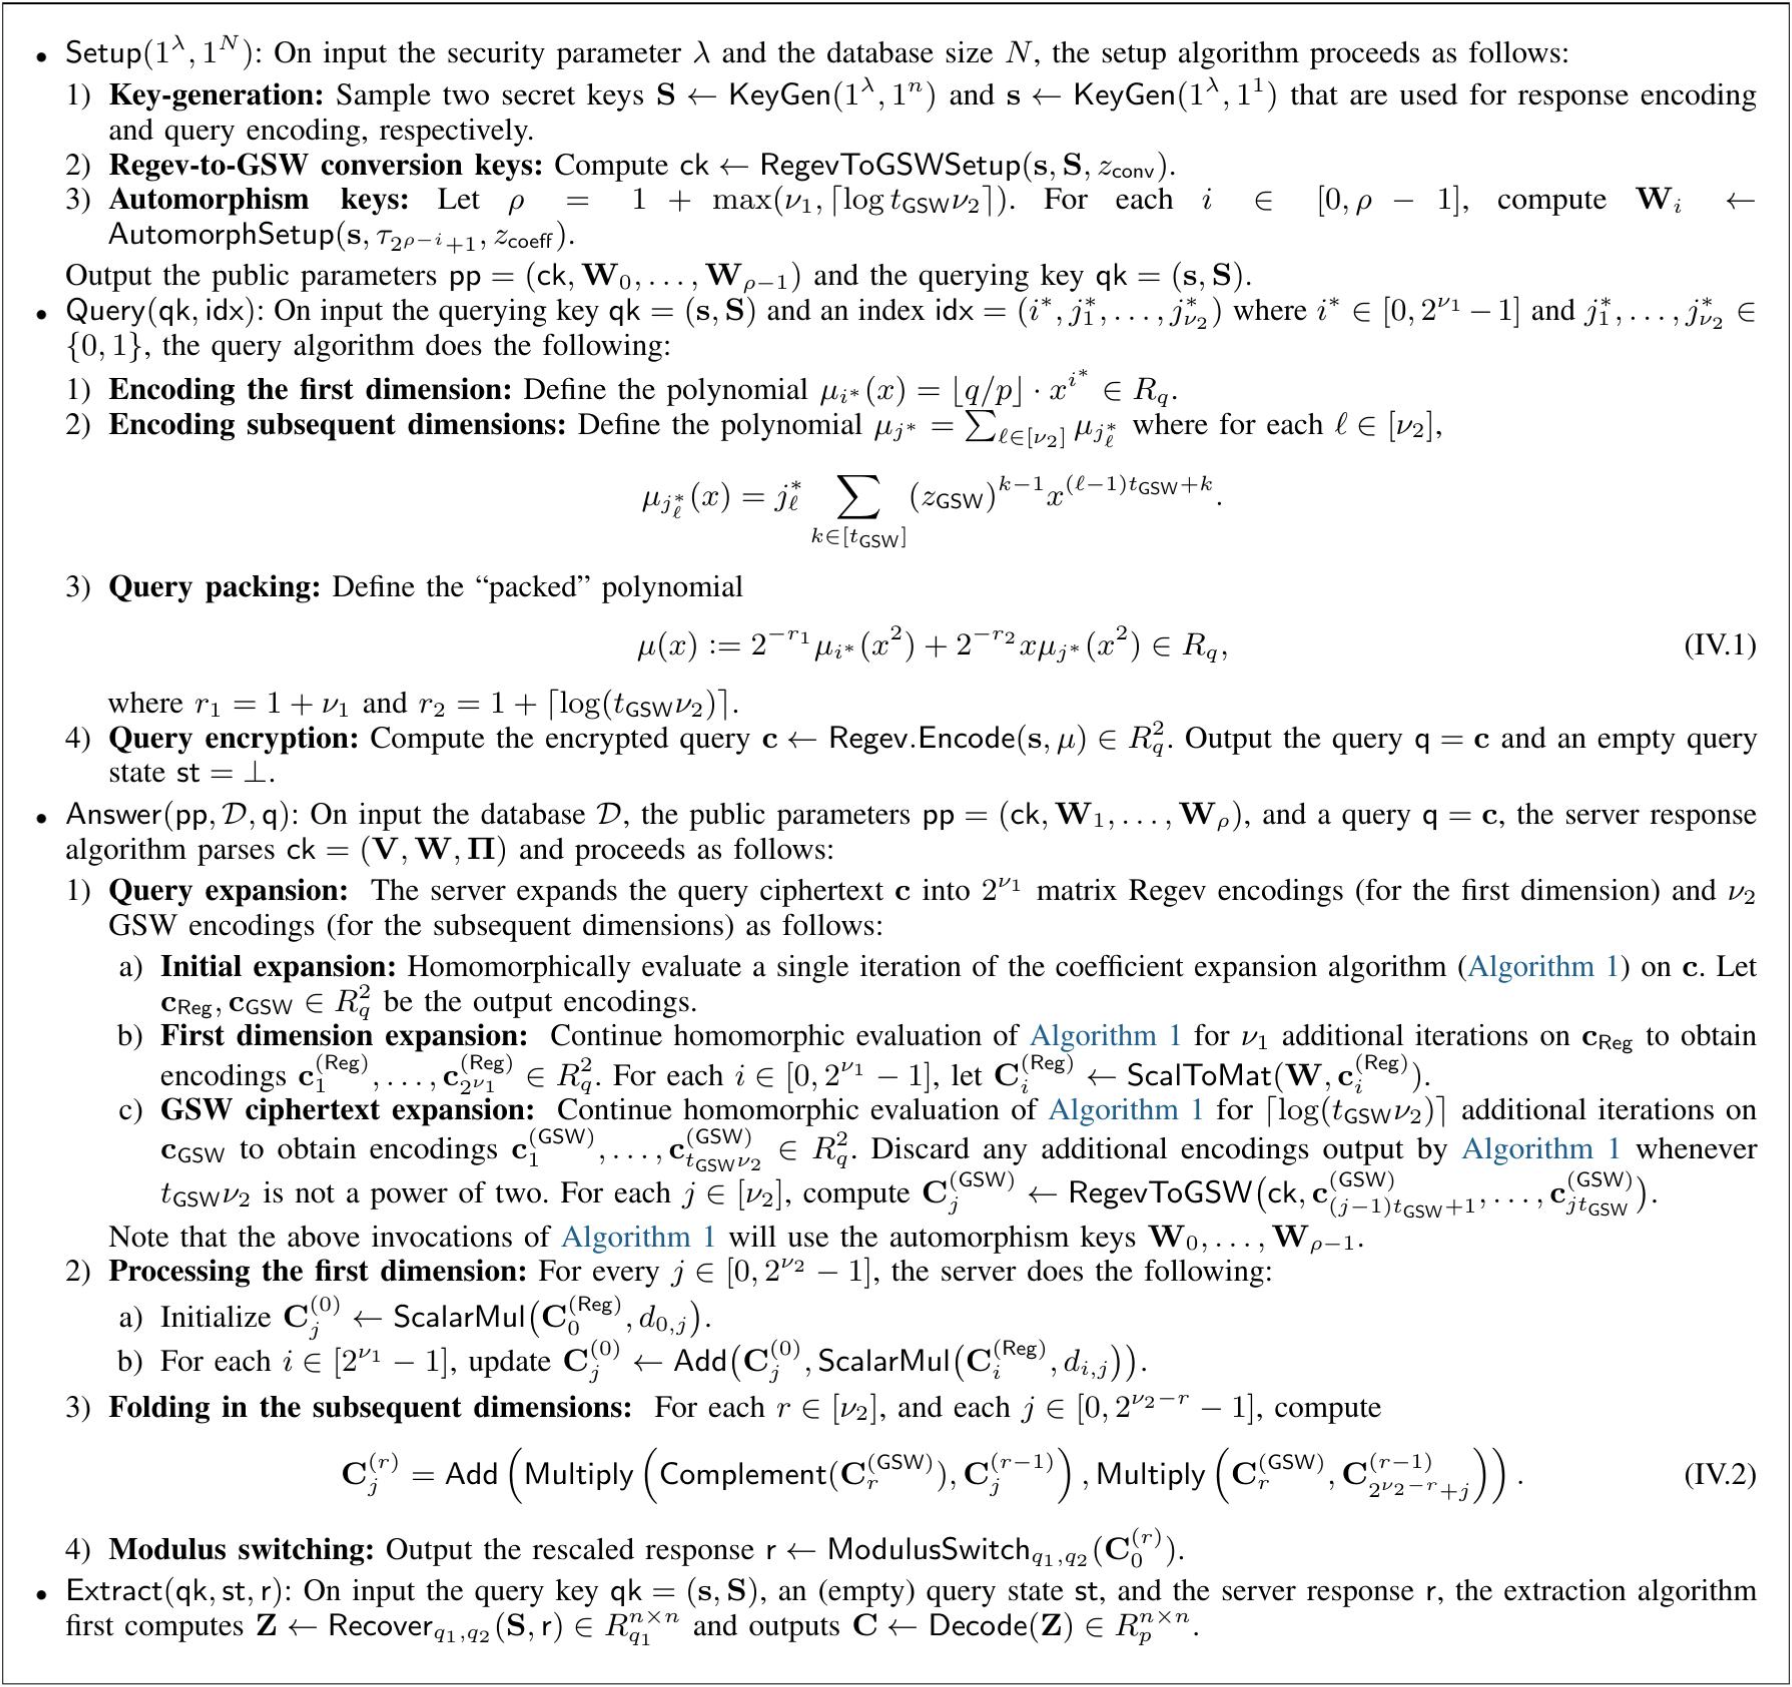
\includegraphics[width=\linewidth]{Images/Spiral_Protocol.png}
    \caption{The SPIRAL PIR protocol.}
    \label{fig:protocol_overview}
\end{figure}
